\documentclass[12pt,a4paper]{article}
\usepackage[utf8]{inputenc}
\usepackage[T1]{fontenc}
%\usepackage[catalan]{babel}
\usepackage{amsmath, amssymb, amsfonts}
\usepackage{graphicx}
\usepackage{url}
\usepackage{comment}
\usepackage{booktabs}
\usepackage{array}
\usepackage[shortlabels]{enumitem}
\usepackage{xcolor}
\usepackage{pgfplots}
\usepackage{tcolorbox}
\usepackage{pdflscape}
\usepackage{makecell}
\usepackage{fancyhdr}
\usepackage[hidelinks]{hyperref}
\usepackage{tocloft}
\usepackage{geometry}
\usepackage{float}
\usepackage{tikz}
\usepackage{listings}
\usepackage{pdfpages}
\usetikzlibrary{trees}
\usetikzlibrary{shapes,arrows,positioning}

\geometry{a4paper, top=2.3cm, bottom=2cm, left=2.3cm, right=2.3cm}

\lstdefinestyle{mystyle}{
    backgroundcolor=\color{backcolour},   
    commentstyle=\color{codegreen},
    keywordstyle=\color{blue},
    numberstyle=\tiny\color{codegray},
    stringstyle=\color{codepurple},
    basicstyle=\ttfamily\small,
    breakatwhitespace=false,         
    breaklines=true,                 
    captionpos=b,                    
    keepspaces=true,                 
    numbers=left,                    
    numbersep=5pt,                  
    showspaces=false,                
    showstringspaces=false,
    showtabs=false,                  
    tabsize=2
}

\definecolor{codegreen}{rgb}{0,0.6,0}
\definecolor{codegray}{rgb}{0.5,0.5,0.5}
\definecolor{codepurple}{rgb}{0.58,0,0.82}
\definecolor{backcolour}{rgb}{0.95,0.95,0.92}

\lstset{style=mystyle}
\lstset{
  literate={á}{{\'a}}1 {é}{{\'e}}1 {í}{{\'i}}1 {ó}{{\'o}}1 {ú}{{\'u}}1
           {ü}{{\"u}}1 {ñ}{{\~n}}1 {ç}{{\c{c}}}1
}

% Define bag style for tikz
\tikzset{bag/.style={rectangle, draw}}

\title{\LARGE IoT Platform}
\author{Aprenentatge i raonament automàtic}
\date{\today}

\pagestyle{fancy}
\fancyhf{}
\fancyhead[L]{GraphQL}
\fancyhead[R]{Distributed computing}

\fancyfoot[C]{\thepage}
\renewcommand{\headrulewidth}{0.4pt}
\renewcommand{\footrulewidth}{0.4pt}

\begin{document}

\begin{titlepage}
  \begin{center}

    \includegraphics[width=5cm]{udl.png}
    \hspace{0.2cm}
    \includegraphics[width=6cm]{eps.jpg}
    
    \vspace{1cm}
    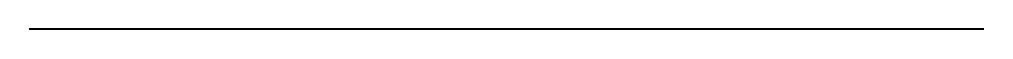
\begin{tikzpicture}[line width=1pt]
      \draw (0,0) -- (\textwidth,0);
    \end{tikzpicture}
    
    \vspace{3cm}
    {\LARGE \textbf{Project 1: Internet of Things applications}}

    \vspace{3cm}
    {\Large Simulate the creation of an IoT platform to gather information,
optimize, and control the climate and comfort of remote homes. Using kafka, MQTT, and InfluxDB.}
    
    \vspace{3cm}
    
    \vfill
    {\Large \today}
    \vfill
    
    \vfill

    {\Large May Castells Raga \par}
    {\Large Anna Marin Nuño \par}
    \vfill
    
    \vspace{1cm}
    {\large Distributed Computing\\}
    {\large Grau en Enginyeria Informàtica\\}
    {\large Universitat de Lleida}
    
    \vspace{1cm}
    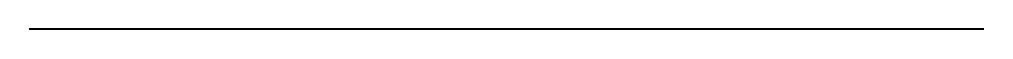
\begin{tikzpicture}[line width=1pt]
      \draw (0,0) -- (\textwidth,0);
    \end{tikzpicture}
  \end{center}
\end{titlepage}
\newpage

% Índice
%\renewcommand{\contentsname}{Índex}
\tableofcontents
\newpage

\section{Brief introduction}

This project simulate the creation of an IoT platform to gather information,
optimize, and control the climate and comfort of remote homes. The project's schhema can be divided into two main parts: the user side and the cloud side.

\section{User / home part}
The user side is composed of several sensors, each one has its own temperature measurement and its own heatpump actuator. Each sensor is represented by a Docker container with a simulating script that generates temperature data.

Each user or home has a MQTT (Message Queuing Telemetry Transport) broker that receives the temperature data from the sensors. In addition, the broker sends commands to the heatpump actuators to adjust the temperature as needed, if the broker receives such commands from the cloud side, it broadcasts them to the corresponding actuators. The MQTT broker is also represented by a Docker container.

The most important component of the user side is the gateway, which is responsible of the communication between the user side and the cloud side. The gateway subscribes to the MQTT broker to receive temperature data from the sensors and publishes the gathered data to the cloud side using another MQTT broker located in the cloud side.
The gateway also deals with the commands received from the cloud side, publishing them to the local MQTT broker so that the actuators can receive them. It subscribes to the cloud MQTT broker to re
The gateway is also represented by a Docker container.

\begin{thebibliography}

\bibitem{polyapi}
PolyAPI. (2023). Darko's Thoughts: GraphQL and REST APIs – What Does the Future Hold? Retrieved October 24, 2025, from \url{https://polyapi.io/darkos-thoughts-graphql-and-rest-apis-what-does-the-future-hold/}

\end{thebibliography}

\begin{comment}
    
\section{Presentation outline}
start with an example right from the beginning 

\begin{enumerate}

\item what we want to do: explain we want to create a API for a social media app, explain which relations in the app db

\item what we are used to do: explain how would be done using Rest

imagine we are in 2012 and we are facebook and want a solution to create an api to retrieve relations of relations

\item introduction, query language and runtime for APIs)., origin facebook 2012

\item motivation, which problem solves

\item concepts, schhema, queries


\item how our example  was build: explain how to create resolvers

\item query language examplea
\item type system as a contract between client and server.

\item single endpoint model vs rest

\item experiment bechmarks

\item advantages 

\item limitations

\item Real-World Use Cases Facebook, GitHub, Shopify, Twitter, etc.

\end{enumerate}



\section{Report Outline}
15 pages
\begin{enumerate}

\item introduction
\item motivation, which problem solves

\item concepts, schhema, queries

\item single endpoint model

\item type system as a contract between client and server.

\item efficiency
\item how internally works
\item how the runtime works
\item some benchmark,  maybe own?
\item advantages 

\item limitations
\item recent changes and future
\item Real-World Use Cases Facebook, GitHub, Shopify, Twitter, etc.

\end{enumerate}

Extra ideas: modify operations and multiapi
\end{comment}

\begin{comment}
    \section{References}
\begin{itemize}
    \item https://graphql.org/learn/\\
    \item https://keepcoding.io/blog/que-es-graphql-y-para-que-sirve/\\
    \item https://apipark.com/techblog/en/top-7-examples-of-graphql-in-action-real-world-use-cases-unveiled/\\
    \item https://medium.com/@ignatovich.dm/graphql-in-2025-pros-cons-public-apis-and-use-cases-part-1-1588cb9e9f9a\\
    \item https://medium.com/@alexisrolland/a-better-way-to-develop-your-graphql-api-using-docker-postgresql-postgraphile-7a1ae034b826
\end{itemize}

\end{comment}


\end{document}



